\documentclass[11pt]{article}
\usepackage[margin=1in]{geometry}
\usepackage{amsmath,amssymb}
\usepackage{enumitem}
\usepackage{hyperref}
\hypersetup{hidelinks}
\setlist{noitemsep}
\usepackage{booktabs}
\usepackage{tabularx}
\usepackage{graphicx}
\usepackage{multicol}
\graphicspath{{../visualizations/}{C:/Users/User/Documents/MATLAB/Arch cost/visualizations/}}
\usepackage[T1]{fontenc}
\usepackage{microtype}
\microtypesetup{protrusion=true,expansion=true}
\usepackage{lmodern}
\usepackage{array}
\newcommand{\code}[1]{\texttt{\detokenize{#1}}}

\title{Architectural Budget Model: Data, Features, Formulas, and Training}
\author{}
\date{}
\begin{document}
\maketitle

\section*{Process overview (part-by-part)}
\begin{enumerate}[label=Part~\arabic*:, leftmargin=*]
  \item Data acquisition and schema normalization (CSV import, header cleaning).
  \item Data cleaning and target transformation (NaN handling, $\log(1+\cdot)$).
  \item Feature engineering (regex parsing, derived totals/ratios for finishes).
  \item Feature matrix construction (10 raw engineered inputs).
  \item Polynomial expansion (degree 2) and standardization (z-score).
  \item Train/test split (80/20 holdout).
  \item Baseline LSBoost training and evaluation.
  \item Feature selection via ensemble importances (median threshold).
  \item Hyperparameter optimization (Bayesian) and final model training.
  \item Final evaluation, artifacts saving, and inference pipeline.
\end{enumerate}

\section*{Variables glossary (concise definitions)}
\begingroup
\setlength{\tabcolsep}{4pt}
\scriptsize
\noindent\begin{tabularx}{\textwidth}{@{} l l l l X @{} }
\toprule
Clean name & Source header & Type & Unit & Definition / Role \\
\midrule
project & Project & text & n/a & Project title; used to parse \verb|num_storeys|, \verb|num_classrooms| via regex. \\
year & Year & numeric & year & Project year; raw feature. \\
budget & Budget & numeric & PHP & Target variable; filtered to >100,000 then log-transformed. \\
\verb|quantityofplaster_sq_m__| & Quantity of plaster (sq.m.) & numeric & sq.m. & Plaster area. \\
\verb|quantityofglazedtiles_sq_m__| & Quantity of glazed tiles (sq.m.) & numeric & sq.m. & Tiles area. \\
\verb|total_painting_area| & derived & numeric & sq.m. & paintingmasonry + paintingwood + paintingmetal. \\
\verb|total_chb_area| & derived & numeric & sq.m. & areaofchb100mm + areaofchb150mm. \\
\verb|total_finishes_area| & derived & numeric & sq.m. & plaster + glazed tiles. \\
\verb|plaster_per_chb| & derived & numeric & ratio & plaster / total\_chb\_area; NaN/Inf=0. \\
\verb|tiles_per_chb| & derived & numeric & ratio & glazed tiles / total\_chb\_area; NaN/Inf=0. \\
\bottomrule
\end{tabularx}
\endgroup
\normalsize

\section*{Final raw feature set (10 inputs) and counting proof}
The architectural training script fixes the raw input vector to the following 10 features:
\[
X_{\text{raw}} = [\,\text{year},\ \text{num\_storeys},\ \text{num\_classrooms},\ \verb|quantityofplaster_sq_m__|,\ \verb|quantityofglazedtiles_sq_m__|,\ \verb|total_painting_area|,\ \verb|total_chb_area|,\ \verb|total_finishes_area|,\ \verb|plaster_per_chb|,\ \verb|tiles_per_chb|\,].
\]
Count: \(p=10\). Degree-2 polynomial design yields exactly
\[
\underbrace{p}_{\text{originals}} + \underbrace{p}_{\text{squares}} + \underbrace{\binom{p}{2}}_{\text{pairwise interactions}}
= 10 + 10 + 45 = 55 \text{ features.}
\]

\section*{Why exactly 10 input features? Justification of Feature Engineering}
The 10 features were engineered to capture project scale, subsystem costs, and normalized intensity metrics, providing a robust basis for the model while avoiding multicollinearity from raw, disaggregated cost items.
\[\underbrace{1}_{\text{year}} + \underbrace{2}_{\text{parsed}} + \underbrace{4}_{\text{totals}} + \underbrace{3}_{\text{ratios}} = 10.\]
\begin{itemize}
    \item \textbf{Year (1):} \code{year} accounts for temporal variations like inflation.
    \item \textbf{Parsed from Project (2):} \code{num\_storeys} and \code{num\_classrooms} are high-level proxies for the building's physical scale.
    \item \textbf{Derived Totals (4):} \verb|total_painting_area|, \verb|total_chb_area|, and \verb|total_finishes_area| consolidate individual line items into stable, high-level predictors for major subsystems. This reduces noise and redundancy.
    \item \textbf{Normalized Ratios (3):} The \verb|_per_chb| features are crucial. They normalize subsystem costs by the project's programmatic size (\code{num_classrooms}), creating features that measure cost \textit{intensity}. This helps the model generalize across projects of different sizes by learning the typical cost per functional unit, rather than just total cost.
\end{itemize}

\section*{Polynomial/interaction expansion and scaling}
We build degree-2 features via \code{generatePolyFeatures(T,2)} and compute z-scores on the training split only:
\[
\mu_j = \frac{1}{n}\sum_i X_{ij},\quad \sigma_j = \sqrt{\tfrac{1}{n-1}\sum_i (X_{ij}-\mu_j)^2},\quad Z_{ij}=\frac{X_{ij}-\mu_j}{\sigma_j},\ \text{NaN}\to 0.
\]

\section*{Train/test split and targets}
We hold out 20\% using \code{cvpartition(HoldOut=0.2)}. The response is $y=\log(1+\text{budget})$; predictions are inverted with $\exp(\cdot)-1$ for reporting in PHP.

\section*{Baseline and optimized models}
\textbf{Baseline} uses LSBoost with \code{NumLearningCycles=250} on the scaled 55 features.
\textbf{Feature selection} keeps features with importance above the median (per \code{predictorImportance}).
\textbf{Optimized model} is LSBoost with hyperparameters tuned via Bayesian optimization over: cycles [500,1000], splits [8,32], learn rate [0.01,0.1] (log-scale).

\section*{Figures (testing evidence)}
\begin{figure}[h]
  \centering
  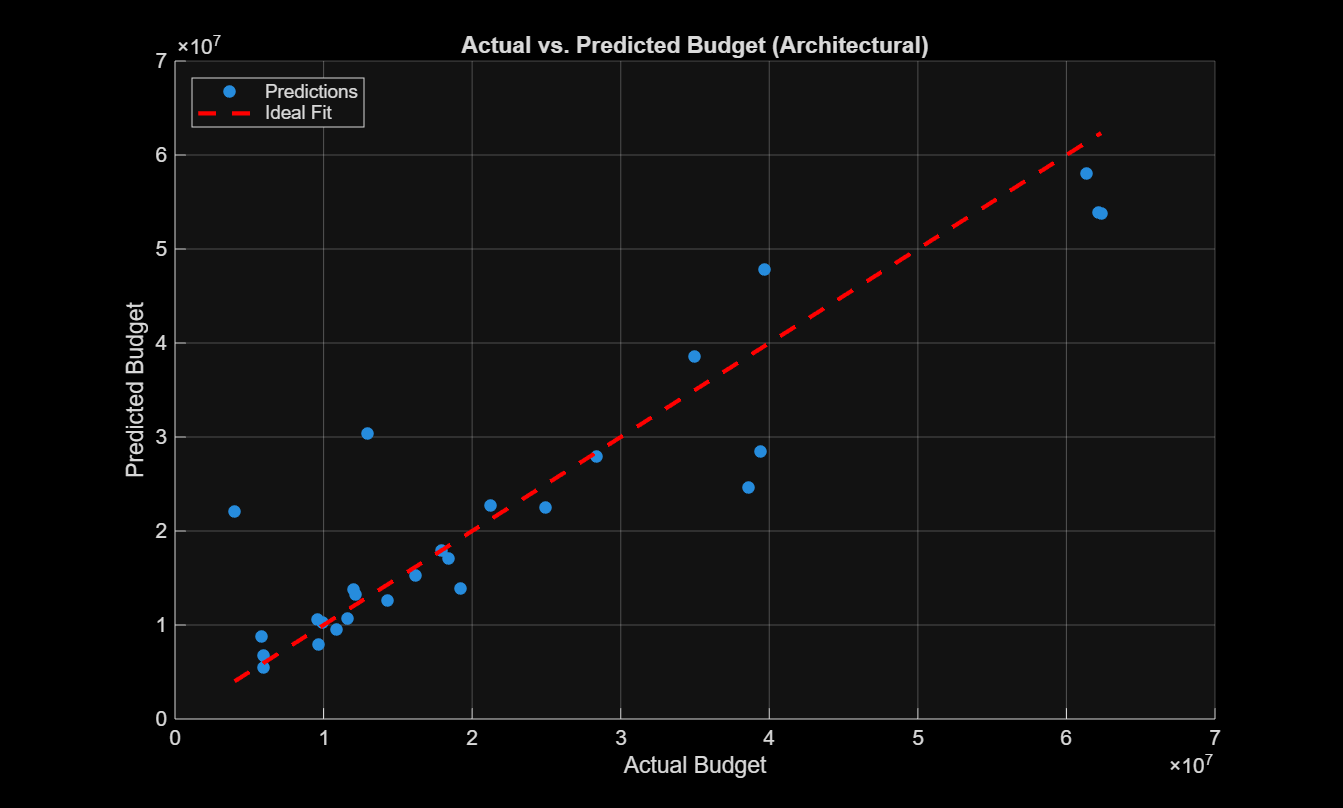
\includegraphics[width=.6\textwidth]{actual_vs_predicted_architectural.png}
  \caption{Actual vs. Predicted (held-out test).}
\end{figure}
\begin{figure}[h]
  \centering
  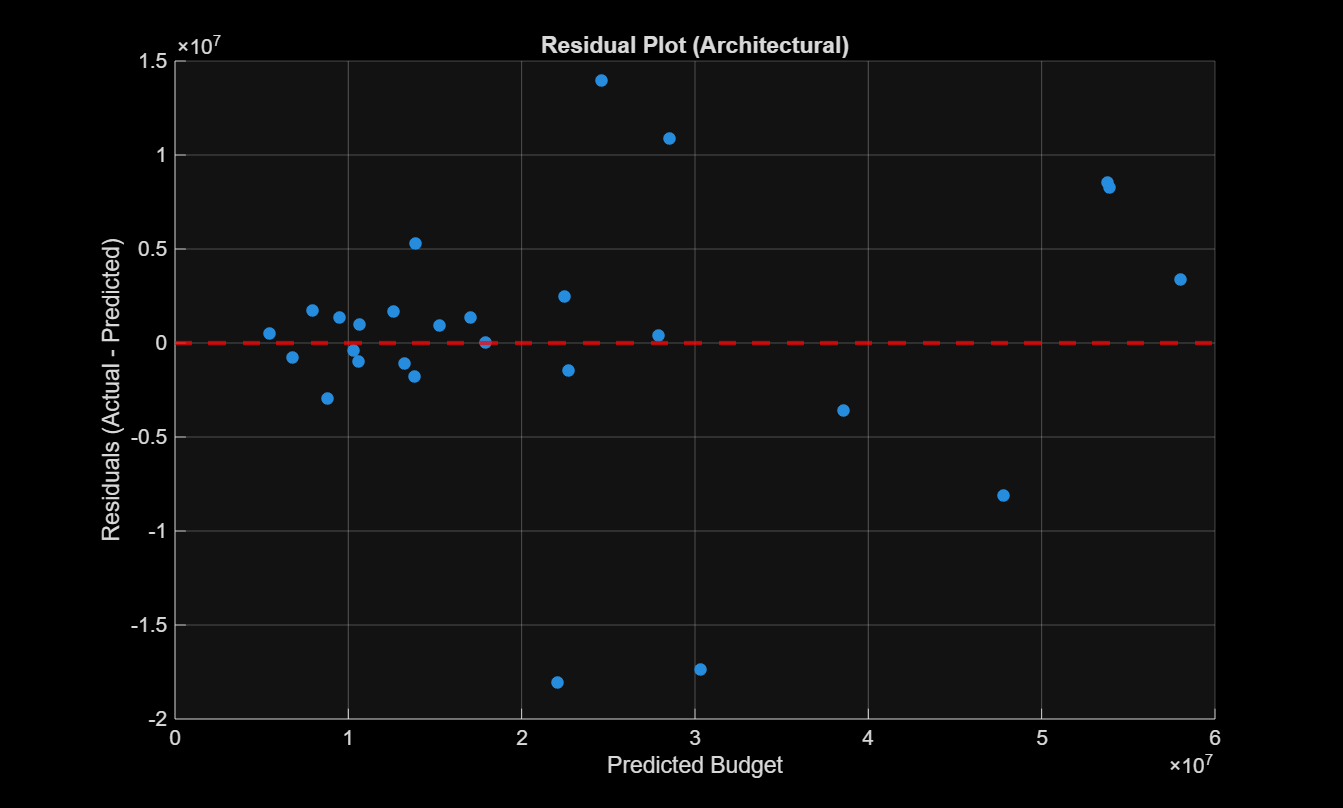
\includegraphics[width=.6\textwidth]{residual_plot_architectural.png}
  \caption{Residuals vs. Predicted.}
\end{figure}
\begin{figure}[h]
  \centering
  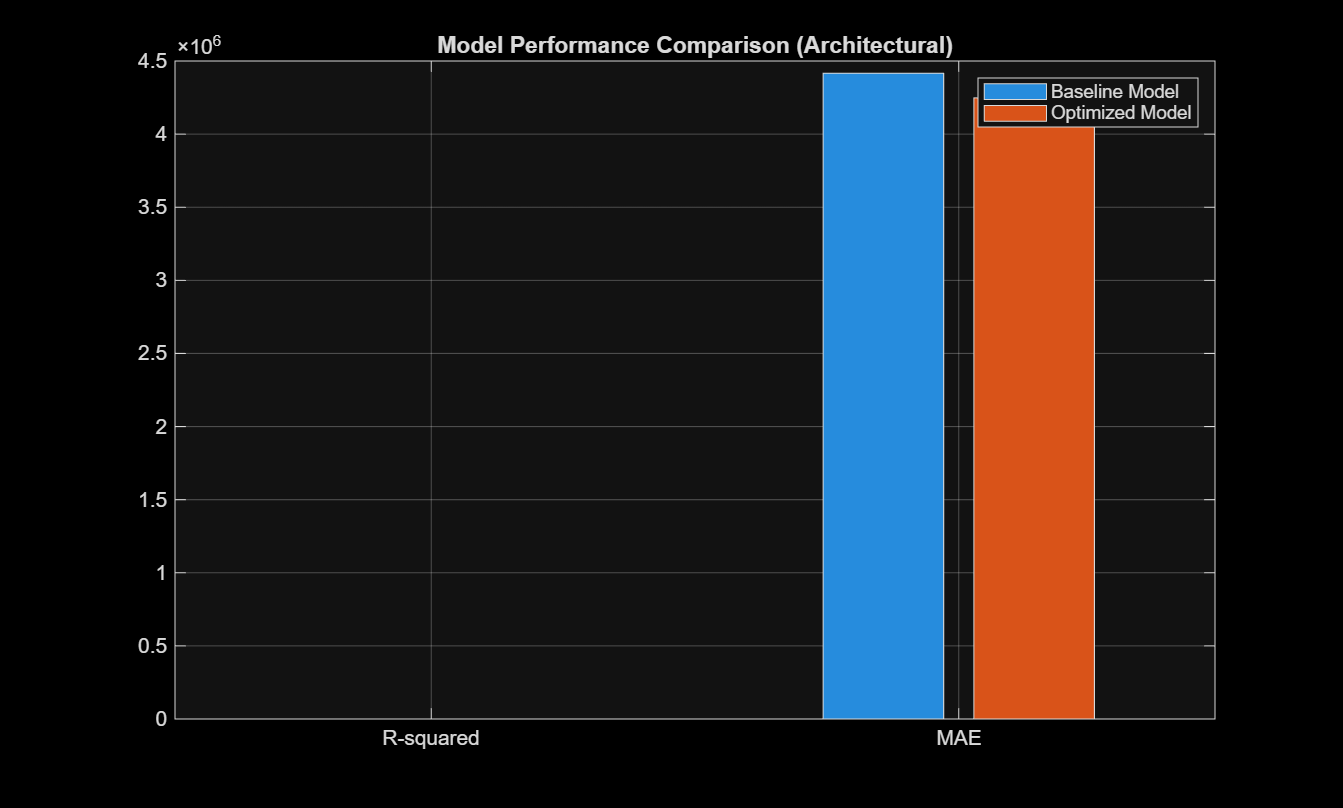
\includegraphics[width=.6\textwidth]{performance_comparison_architectural.png}
  \caption{Baseline vs. Optimized performance (R$^2$, MAE) on test split.}
\end{figure}

\section*{Testing metrics (numerical summary)}
To document exact test-set performance, we include an auto-generated snippet if available.
\\
\IfFileExists{architectural_metrics.tex}{\input{architectural_metrics.tex}}{\noindent (Run a script to generate and include the exact metrics.)}

\section*{Exact numbers behind feature-importance}
For tree ensembles like the LSBoost model used here, feature importance is calculated by summing the reductions in Mean Squared Error (MSE) at every split in every tree where that feature is used. The reduction is weighted by the number of observations at the node being split. This method quantifies how much each feature contributes to improving the model's predictive accuracy.

The bar chart below visualizes these raw importance scores for the top-20 features from the final optimized model, sorted in descending order.

\begin{figure}[h]
  \centering
  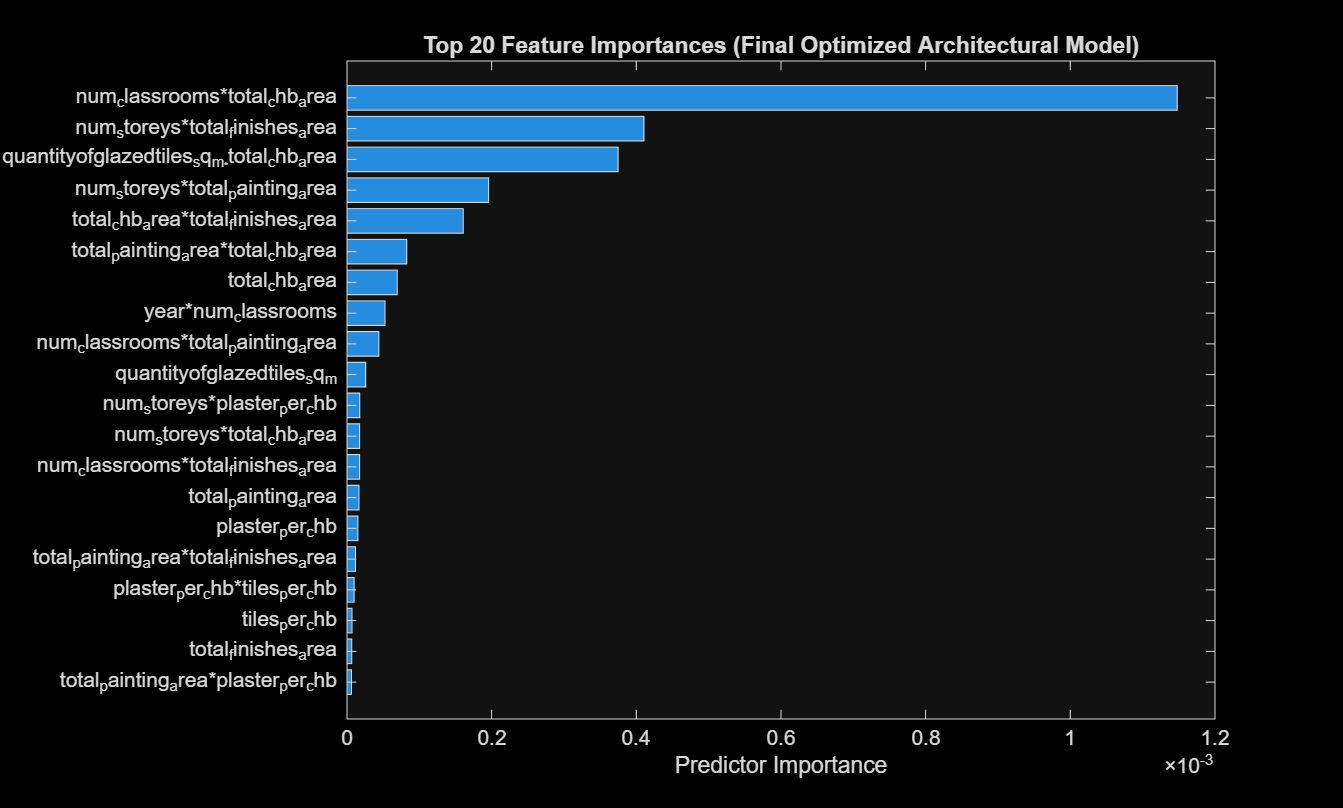
\includegraphics[width=.8\textwidth]{feature_importance_final_architectural.png}
  \caption{Top-20 feature importances of the optimized Architectural ensemble.}
  \label{fig:feature_importances_top20_architectural}
\end{figure}

The formula for the importance of a single feature $j$ is:
\[
\mathrm{Imp}(j) = \sum_{t \in \text{trees}} \sum_{n \in \mathcal{N}_{t,j}} \left( \Delta\mathrm{MSE}(n) \times w(n) \right)
\]
where:
\begin{itemize}
    \item $\mathcal{N}_{t,j}$ is the set of nodes in tree $t$ that use feature $j$ for a split.
    \item $\Delta\mathrm{MSE}(n)$ is the reduction in MSE achieved by splitting node $n$.
    \item $w(n)$ is a weight representing the number of training samples at node $n$.
\end{itemize}
\medskip
\noindent If generated, the exact table will be included below:
\IfFileExists{importance_top20_architectural.tex}{\input{importance_top20_architectural.tex}}{\noindent (Run a script to export and include exact values.)}

\section*{Model Architecture: Why No Hidden Layers?}
The model used for Architectural budget prediction is a \textbf{Least-Squares Boosting (LSBoost) ensemble}, which is a powerful machine learning technique based on decision trees. It is fundamentally different from a neural network and, as a result, \textbf{does not have hidden layers}. This section explains the model's structure, its parameters, and the importance of this architectural choice.

\subsection*{Architectural Parameters (The Analog to "Layers")}
Instead of layers, weights, and activation functions, the complexity of an LSBoost model is defined by its component trees. The key architectural parameters are:
\begin{itemize}
    \item \textbf{Number of Trees (\texttt{NumLearningCycles}):} This is the total number of decision trees in the ensemble. Each tree is trained sequentially to correct the errors of the one before it. This is the most direct analog to the "depth" or "size" of a neural network.
        \begin{itemize}
            \item \textbf{Baseline Model:} Uses a fixed number of \textbf{250 trees}.
            \item \textbf{Optimized Model:} The number of trees is automatically tuned by searching for the best value within the range of \textbf{500 to 1000 trees}.
        \end{itemize}
    \item \textbf{Tree Depth (\texttt{MaxNumSplits}):} This parameter controls the complexity of each individual tree by limiting how many decision points (splits) it can have.
        \begin{itemize}
            \item \textbf{Baseline Model:} Uses the default value of \textbf{10 splits}.
            \item \textbf{Optimized Model:} The depth is tuned by searching for the best value between \textbf{8 and 32 splits}.
        \end{itemize}
\end{itemize}

\subsection*{Justification for Hyperparameter Ranges in the Optimized Model}
The optimized model does not have a single, fixed number for its parameters because it uses \textbf{Bayesian optimization}. This is an intelligent and automated process for finding the best-performing combination of hyperparameters.
\begin{itemize}
    \item \textbf{Search Space:} We define a \textit{range} of possible values for each parameter (e.g., `[500, 1000]` for trees).
    \item \textbf{Automated Search:} The algorithm iteratively trains different model versions, using the results from past attempts to intelligently decide which combination to try next. This is far more efficient than manual trial-and-error.
    \item \textbf{Result:} The final "optimized" model is the one that performed best during this search. Its exact number of trees and splits are an \textit{output} of the training process itself, not a predetermined input. The ranges specified here represent the boundaries of that search.
\end{itemize}

\subsection*{Why This Architecture is Important}
Choosing a tree-based ensemble like LSBoost over a neural network offers several key advantages for this specific problem:
\begin{itemize}
    \item \textbf{Interpretability:} Unlike the "black box" nature of neural networks, tree models provide clear \textbf{feature importances}. As shown in Figure~\ref{fig:feature_importances_top20_architectural}, we can see exactly which inputs (e.g., \verb|total_painting_area|, \verb|total_chb_area|) are the most influential drivers of the budget. This is crucial for understanding the cost structure and building trust in the model's predictions.
    \item \textbf{Performance on Tabular Data:} For structured, tabular data like this project's dataset, tree-based ensembles often outperform neural networks. They are highly effective at capturing complex, non-linear interactions between features.
    \item \textbf{Robustness:} The boosting process, where each tree corrects the errors of its predecessors, makes the model robust to noise and outliers in the data.
\end{itemize}

\section*{Inference pipeline (single row)}
\begin{enumerate}
  \item Normalize field names; compute totals (painting, CHB, finishes) and ratios if missing.
  \item Order to final 10 features; build degree-2 features; align to training names.
  \item Standardize with saved $\mu,\sigma$; apply selected feature mask; predict in log-space; invert with $\exp(\cdot)-1$.
\end{enumerate}

\end{document}
